% ==========================================================================
% INFO 4617 Web Data Science -- Week 2: Ethics, Law & Responsible Data
% Collection (Chapter 2)
% Build:  latexmk -pdf week-02.tex   (from this folder; no env vars needed)
% (or run `make` from the slides/ directory to build every deck)
% ==========================================================================
\documentclass[9pt,aspectratio=169]{beamer}
% Resolve the shared theme/preamble in ../common/ when compiling this
% file directly from its own folder (no TEXINPUTS needed).
\makeatletter\def\input@path{{../common/}}\makeatother
% ==========================================================================
% Shared preamble for INFO 4617 Web Data Science weekly lecture decks
% Based on the Gotham beamer theme (vendored in this directory).
% Each week's slides.tex does:  % ==========================================================================
% Shared preamble for INFO 4617 Web Data Science weekly lecture decks
% Based on the Gotham beamer theme (vendored in this directory).
% Each week's slides.tex does:  % ==========================================================================
% Shared preamble for INFO 4617 Web Data Science weekly lecture decks
% Based on the Gotham beamer theme (vendored in this directory).
% Each week's slides.tex does:  \input{preamble}  (with common/ on TEXINPUTS)
% then sets \title/\subtitle/\author/\date and \begin{document}.
% ==========================================================================

\usetheme{gotham}

\usepackage{fbb}
\usepackage{booktabs}
\usepackage{graphicx}
\usepackage{tikz}
\usepackage{xcolor}
\usepackage{multirow}
\usepackage{listings}
\usetikzlibrary{positioning, arrows.meta, shapes}

% Bibliography
\usepackage[style=authoryear,
            backend=biber,
            maxcitenames=1,
            uniquename=false,
            uniquelist=false]{biblatex}
\addbibresource{bibliography.bib}

\gothamset{sectiontocframe default=off}

% ------------------------------------------------------------------ colors
\definecolor{cugold}{HTML}{CFB87C}
\definecolor{tab-red}{HTML}{E15759}
\definecolor{tab-orange}{HTML}{F28E2B}
\definecolor{tab-blue}{HTML}{4E79A7}
\definecolor{tab-cyan}{HTML}{76B7B2}
\definecolor{tab-green}{HTML}{59A14F}
\definecolor{tab-yellow}{HTML}{EDC948}
\definecolor{tab-purple}{HTML}{B07AA1}
\definecolor{tab-pink}{HTML}{FF9DA7}
\definecolor{tab-brown}{HTML}{9C755F}
\definecolor{tab-gray}{HTML}{BAB0AC}

\setbeamercolor{frametitle}{fg=black, bg=cugold}
\setbeamercolor{progress bar}{fg=cugold, bg=cugold!20}

\setbeamercolor{block title alerted}{fg=black, bg=cugold}
\setbeamercolor{block body alerted}{fg=black, bg=cugold!10}

% ------------------------------------------------------------------ footline
\setbeamertemplate{footline}{
  \begin{beamercolorbox}[wd=\paperwidth,ht=2.5ex,dp=1ex,right]{footline}
    {\footnotesize \insertframenumber{} of \inserttotalframenumber}
    \hspace*{2ex}
  \end{beamercolorbox}
}

% ------------------------------------------------------------------ helpers
\newcommand{\bottomcite}[1]{
    \vspace*{\fill}
    \vspace{-\baselineskip}
    {\tiny
    \rule{\textwidth}{0.3pt}\\
    #1
    }
    \vspace{0.5ex}
}

% Consistent code styling for the Wednesday "applied notebook" frames.
\lstdefinestyle{wds}{
    basicstyle=\ttfamily\scriptsize,
    keywordstyle=\color{tab-blue}\bfseries,
    commentstyle=\color{tab-green},
    stringstyle=\color{tab-orange},
    showstringspaces=false,
    breaklines=true,
    columns=fullflexible,
    language=Python,
    aboveskip=0.4em,
    belowskip=0.4em,
}
\lstset{style=wds}

% \dayband{Day}{Topic} -- a lightweight section divider label used to mark
% Monday / Wednesday / Friday within a week's deck.
\newcommand{\dayband}[2]{{\large\textbf{#1}}\;\textcolor{tab-gray}{\textbar}\;#2}
  (with common/ on TEXINPUTS)
% then sets \title/\subtitle/\author/\date and \begin{document}.
% ==========================================================================

\usetheme{gotham}

\usepackage{fbb}
\usepackage{booktabs}
\usepackage{graphicx}
\usepackage{tikz}
\usepackage{xcolor}
\usepackage{multirow}
\usepackage{listings}
\usetikzlibrary{positioning, arrows.meta, shapes}

% Bibliography
\usepackage[style=authoryear,
            backend=biber,
            maxcitenames=1,
            uniquename=false,
            uniquelist=false]{biblatex}
\addbibresource{bibliography.bib}

\gothamset{sectiontocframe default=off}

% ------------------------------------------------------------------ colors
\definecolor{cugold}{HTML}{CFB87C}
\definecolor{tab-red}{HTML}{E15759}
\definecolor{tab-orange}{HTML}{F28E2B}
\definecolor{tab-blue}{HTML}{4E79A7}
\definecolor{tab-cyan}{HTML}{76B7B2}
\definecolor{tab-green}{HTML}{59A14F}
\definecolor{tab-yellow}{HTML}{EDC948}
\definecolor{tab-purple}{HTML}{B07AA1}
\definecolor{tab-pink}{HTML}{FF9DA7}
\definecolor{tab-brown}{HTML}{9C755F}
\definecolor{tab-gray}{HTML}{BAB0AC}

\setbeamercolor{frametitle}{fg=black, bg=cugold}
\setbeamercolor{progress bar}{fg=cugold, bg=cugold!20}

\setbeamercolor{block title alerted}{fg=black, bg=cugold}
\setbeamercolor{block body alerted}{fg=black, bg=cugold!10}

% ------------------------------------------------------------------ footline
\setbeamertemplate{footline}{
  \begin{beamercolorbox}[wd=\paperwidth,ht=2.5ex,dp=1ex,right]{footline}
    {\footnotesize \insertframenumber{} of \inserttotalframenumber}
    \hspace*{2ex}
  \end{beamercolorbox}
}

% ------------------------------------------------------------------ helpers
\newcommand{\bottomcite}[1]{
    \vspace*{\fill}
    \vspace{-\baselineskip}
    {\tiny
    \rule{\textwidth}{0.3pt}\\
    #1
    }
    \vspace{0.5ex}
}

% Consistent code styling for the Wednesday "applied notebook" frames.
\lstdefinestyle{wds}{
    basicstyle=\ttfamily\scriptsize,
    keywordstyle=\color{tab-blue}\bfseries,
    commentstyle=\color{tab-green},
    stringstyle=\color{tab-orange},
    showstringspaces=false,
    breaklines=true,
    columns=fullflexible,
    language=Python,
    aboveskip=0.4em,
    belowskip=0.4em,
}
\lstset{style=wds}

% \dayband{Day}{Topic} -- a lightweight section divider label used to mark
% Monday / Wednesday / Friday within a week's deck.
\newcommand{\dayband}[2]{{\large\textbf{#1}}\;\textcolor{tab-gray}{\textbar}\;#2}
  (with common/ on TEXINPUTS)
% then sets \title/\subtitle/\author/\date and \begin{document}.
% ==========================================================================

\usetheme{gotham}

\usepackage{fbb}
\usepackage{booktabs}
\usepackage{graphicx}
\usepackage{tikz}
\usepackage{xcolor}
\usepackage{multirow}
\usepackage{listings}
\usetikzlibrary{positioning, arrows.meta, shapes}

% Bibliography
\usepackage[style=authoryear,
            backend=biber,
            maxcitenames=1,
            uniquename=false,
            uniquelist=false]{biblatex}
\addbibresource{bibliography.bib}

\gothamset{sectiontocframe default=off}

% ------------------------------------------------------------------ colors
\definecolor{cugold}{HTML}{CFB87C}
\definecolor{tab-red}{HTML}{E15759}
\definecolor{tab-orange}{HTML}{F28E2B}
\definecolor{tab-blue}{HTML}{4E79A7}
\definecolor{tab-cyan}{HTML}{76B7B2}
\definecolor{tab-green}{HTML}{59A14F}
\definecolor{tab-yellow}{HTML}{EDC948}
\definecolor{tab-purple}{HTML}{B07AA1}
\definecolor{tab-pink}{HTML}{FF9DA7}
\definecolor{tab-brown}{HTML}{9C755F}
\definecolor{tab-gray}{HTML}{BAB0AC}

\setbeamercolor{frametitle}{fg=black, bg=cugold}
\setbeamercolor{progress bar}{fg=cugold, bg=cugold!20}

\setbeamercolor{block title alerted}{fg=black, bg=cugold}
\setbeamercolor{block body alerted}{fg=black, bg=cugold!10}

% ------------------------------------------------------------------ footline
\setbeamertemplate{footline}{
  \begin{beamercolorbox}[wd=\paperwidth,ht=2.5ex,dp=1ex,right]{footline}
    {\footnotesize \insertframenumber{} of \inserttotalframenumber}
    \hspace*{2ex}
  \end{beamercolorbox}
}

% ------------------------------------------------------------------ helpers
\newcommand{\bottomcite}[1]{
    \vspace*{\fill}
    \vspace{-\baselineskip}
    {\tiny
    \rule{\textwidth}{0.3pt}\\
    #1
    }
    \vspace{0.5ex}
}

% Consistent code styling for the Wednesday "applied notebook" frames.
\lstdefinestyle{wds}{
    basicstyle=\ttfamily\scriptsize,
    keywordstyle=\color{tab-blue}\bfseries,
    commentstyle=\color{tab-green},
    stringstyle=\color{tab-orange},
    showstringspaces=false,
    breaklines=true,
    columns=fullflexible,
    language=Python,
    aboveskip=0.4em,
    belowskip=0.4em,
}
\lstset{style=wds}

% \dayband{Day}{Topic} -- a lightweight section divider label used to mark
% Monday / Wednesday / Friday within a week's deck.
\newcommand{\dayband}[2]{{\large\textbf{#1}}\;\textcolor{tab-gray}{\textbar}\;#2}


\title[Week 2 · Ethics \& Law]{{\Huge Ethics, Law \& Responsible Data Collection}}
\subtitle{Week 2 · Foundations module · Textbook Chapter 2}
\author[Keegan]{\textbf{Brian C. Keegan, Ph.D.} \\ Associate Professor, Department of Information Science \\ University of Colorado Boulder}
\date{August 24, 26 \& 28, 2026}

\begin{document}

\maketitle

% -------------------------------------------------------------------------
\begin{frame}{This week at a glance}
    \begin{columns}[T]
        \begin{column}{0.6\textwidth}
            Before we collect a single row, we settle the harder question --- not \textit{can} we, but \textbf{should} we, and if so, how responsibly?

            \bigskip

            \dayband{Monday}{Concepts \& notebook intro}
            \begin{itemize}\small
                \item The legal landscape, \texttt{robots.txt}, and a five-question ethical framework
            \end{itemize}

            \medskip

            \dayband{Wednesday}{Notebook lab}
            \begin{itemize}\small
                \item \texttt{robots.txt}, User-Agent headers, rate limiting --- and building \texttt{responsible\_get()}
            \end{itemize}

            \medskip

            \dayband{Friday}{Textbook revisions}
            \begin{itemize}\small
                \item GitHub, hands-on --- and everyone files their first issue against Chapter 2
            \end{itemize}
        \end{column}
        \begin{column}{0.35\textwidth}
            \begin{block}{Companion notebook}
                \footnotesize \texttt{ch-02-ethics.ipynb}
            \end{block}
            \begin{alertblock}{Bring a laptop}
                \footnotesize Wednesday is hands-on --- we send live requests and watch what the server sees.
            \end{alertblock}
        \end{column}
    \end{columns}
\end{frame}

% =========================================================================
\section{Monday · Concepts}
% =========================================================================

\begin{frame}{Monday at a glance}
    \begin{columns}[T]
        \begin{column}{0.6\textwidth}
            \begin{tabular}{@{}ll@{}}
                \textbf{00:00 -- 00:04} & The ethics of retrieval \\[0.3em]
                \textbf{00:04 -- 00:20} & The law: the CFAA, four rulings, \\
                                        & and what is still moving \\[0.3em]
                \textbf{00:20 -- 00:26} & Terms of Service \& privacy policies \\[0.3em]
                \textbf{00:26 -- 00:34} & \textbf{Activity}: audit a platform you use \\[0.3em]
                \textbf{00:34 -- 00:44} & \textbf{Discussion}: four dispatches from \\
                                        & the scraping wars \\[0.3em]
                \textbf{00:44 -- 00:50} & The framework, and Wednesday \\
            \end{tabular}
        \end{column}
        \begin{column}{0.35\textwidth}
            \begin{alertblock}{Two things to have open}
                \footnotesize A browser, and the four articles from the reading. Half of today is you reading primary sources --- not me talking.
            \end{alertblock}
        \end{column}
    \end{columns}
\end{frame}

\begin{frame}{The ethics of retrieval}
    \begin{columns}[T]
        \begin{column}{0.6\textwidth}
            ``Web scraping'' is a popular phrase --- and a faintly pejorative one. Data is \textbf{valuable}: other people invested time, money, and effort to create and host what you are about to retrieve programmatically.

            \bigskip

            So the question is never simply \textbf{``can I scrape this?''} but \textbf{``should I --- and if so, how do I do it responsibly?''}

            \bigskip

            This chapter builds a \textbf{decision framework} to revisit before every collection project in this course and beyond. Three layers of guidance, none sufficient alone: \textbf{law}, \textbf{technical norms} (\texttt{robots.txt}), and \textbf{ethics}.
        \end{column}
        \begin{column}{0.35\textwidth}
            \begin{alertblock}{One idea to carry all semester}
                \footnotesize ``It's technically possible'' is not the same as ``it's legal,'' and ``it's legal'' is not the same as ``it's ethical.''
            \end{alertblock}
        \end{column}
    \end{columns}
    \bottomcite{Textbook Ch.~2, ``The Ethics of Retrieval.''}
\end{frame}

\begin{frame}{The CFAA: a 1986 law meets the modern web}
    \begin{columns}[T]
        \begin{column}{0.6\textwidth}
            The \textbf{Computer Fraud and Abuse Act} was enacted in 1986, expanding a narrower 1984 statute, during a national panic about ``computer crime.'' The web did not exist.

            \medskip

            Its key provision prohibits \textbf{``unauthorized access''} to a computer system. What the statute never does is say what makes access to a \textit{public web page} unauthorized.

            \medskip

            That gap matters because the CFAA is a \textbf{criminal} statute. The question ``was that authorized?'' is not an abstraction --- it is the difference between a research method and a federal charge.

            \medskip

            Forty years of litigation have been an argument about that one word.
        \end{column}
        \begin{column}{0.35\textwidth}
            \begin{alertblock}{Why you should care}
                \footnotesize Every collection decision you make this semester sits underneath a criminal statute drafted before the web existed --- and interpreted by courts that are still disagreeing.
            \end{alertblock}
        \end{column}
    \end{columns}
    \bottomcite{Textbook Ch.~2, ``The Computer Fraud and Abuse Act.''}
\end{frame}

\begin{frame}{Two events that shaped everything after}
    \begin{columns}[T]
        \begin{column}{0.6\textwidth}
            \textbf{Aaron Swartz (2011--2013).} Swartz used MIT's network to bulk-download academic articles from JSTOR. Federal prosecutors charged him under the CFAA --- eleven counts, decades of theoretical exposure --- on a theory that violating a terms-of-use agreement was ``unauthorized access.'' He died by suicide in 2013, at 26.

            \medskip

            \textbf{Cambridge Analytica (2018).} A researcher collected Facebook data through the platform's API for ostensibly academic purposes, then handed it to a political consulting firm. The fallout closed APIs across the industry --- for everyone, including the researchers who had done nothing wrong.
        \end{column}
        \begin{column}{0.35\textwidth}
            \begin{block}{One shock each way}
                \footnotesize \textbf{Swartz} taught researchers that a vague statute could be aimed at them.

                \smallskip

                \textbf{Cambridge Analytica} taught platforms that open access was a liability.

                \smallskip

                Together they explain why the doors were closing before AI ever showed up (Ch.~3).
            \end{block}
        \end{column}
    \end{columns}
    \bottomcite{Textbook Ch.~2, ``Social History and Public Interest.'' On the CFAA's use against researchers: \textcite{fiesler2020no}.}
\end{frame}

\begin{frame}{\textit{Van Buren v.\ United States} (2021)}
    \begin{columns}[T]
        \begin{column}{0.6\textwidth}
            \textbf{The facts.} A police sergeant ran a license-plate search in a database he was \textit{authorized} to use --- but did it for a bribe, not police work. He was charged under the CFAA's ``exceeds authorized access'' clause.

            \medskip

            \textbf{The holding.} The Supreme Court adopted a \textbf{``gates-up-or-down''} reading: the CFAA targets entering areas you are not entitled to enter. It does \textit{not} reach misusing information you were allowed to see.

            \medskip

            \textbf{Why it matters to you.} Before \textit{Van Buren}, a prosecutor could plausibly argue that breaking a website's stated terms was a federal crime. After it, that theory is very hard to sustain.
        \end{column}
        \begin{column}{0.35\textwidth}
            \begin{block}{The test, in one line}
                \footnotesize Did you go \textbf{around a gate}, or did you break a \textbf{rule} about data you could already reach?

                \smallskip

                Only the first is the CFAA's business.
            \end{block}
        \end{column}
    \end{columns}
    \bottomcite{Textbook Ch.~2, ``Legal Frameworks.'' A gate is authentication --- a login, a paywall, an API key.}
\end{frame}

\begin{frame}{\textit{hiQ Labs v.\ LinkedIn} (2019--2022): read the whole arc}
    \begin{columns}[T]
        \begin{column}{0.6\textwidth}
            This is the case people cite \textit{wrong}. It has three acts:
            \begin{enumerate}\small
                \item hiQ, an analytics company, scraped \textbf{public} LinkedIn profiles. LinkedIn sent a cease-and-desist and blocked it.
                \item The Ninth Circuit held --- in 2019, and \textbf{again in 2022} after the Supreme Court sent it back in light of \textit{Van Buren} --- that scraping publicly accessible data likely does \textbf{not} violate the CFAA. No authentication gate was bypassed.
                \item Later in 2022, hiQ \textbf{lost} on LinkedIn's \textbf{breach-of-contract} claim: it kept scraping after agreeing to the ToS and receiving the C\&D. The case settled with hiQ agreeing to stop.
            \end{enumerate}
        \end{column}
        \begin{column}{0.35\textwidth}
            \begin{alertblock}{The half-quote}
                \footnotesize You will hear ``\textit{hiQ} means scraping public data is legal.''

                \smallskip

                That is act two of three. The company still lost, and stopped scraping.

                \smallskip

                \textbf{The CFAA is not the only law in the room.}
            \end{alertblock}
        \end{column}
    \end{columns}
    \bottomcite{Textbook Ch.~2, ``Legal Frameworks.'' Criminal exposure and contractual exposure are different questions with different answers.}
\end{frame}

\begin{frame}{\textit{Sandvig v.\ Barr} (2020)}
    \begin{columns}[T]
        \begin{column}{0.6\textwidth}
            \textbf{The facts.} Researchers wanted to run \textbf{audit studies} of algorithmic discrimination --- creating test profiles on housing and employment sites to see whether the algorithms treated them differently by race. Doing that violates those sites' Terms of Service. Fearing CFAA prosecution, they sued \textit{first}.

            \medskip

            \textbf{The holding.} A federal district court held in 2020 that merely violating a website's Terms of Service is \textbf{not} a CFAA crime.

            \medskip

            \textbf{Why it matters.} Audit studies are how we know what we know about algorithmic discrimination. This ruling is modest --- one district court --- but it is real cover for a whole research method.
        \end{column}
        \begin{column}{0.35\textwidth}
            \begin{block}{The tension it names}
                \footnotesize Platforms write the rules that govern how they may be studied.

                \smallskip

                A ToS that forbids test accounts is also a ToS that forbids auditing you for discrimination.
            \end{block}
        \end{column}
    \end{columns}
    \bottomcite{Textbook Ch.~2, ``Legal Frameworks.'' Audit methodology and ToS restrictions: \textcite{fiesler2020no}.}
\end{frame}

\begin{frame}{Four rulings, one through-line}
    \begin{center}\small
    \begin{tabular}{@{}p{0.20\textwidth}p{0.36\textwidth}p{0.36\textwidth}@{}}
        \toprule
        \textbf{Case} & \textbf{Holding} & \textbf{What it means for you} \\
        \midrule
        \textit{Van Buren} (2021) & CFAA reaches gates, not use restrictions & Breaking a rule $\neq$ a federal crime \\
        \textit{hiQ} (2019, 2022) & Public scraping likely not CFAA --- but breach of contract & Winning on the CFAA is not winning \\
        \textit{Sandvig} (2020) & ToS violation alone is not a CFAA crime & Audit research has some cover \\
        \textit{Bright Data} (2024) & Logged-out public scraping survived contract claims & Never agreeing means no contract \\
        \bottomrule
    \end{tabular}
    \end{center}
    \medskip
    {\footnotesize \textbf{The through-line:} the CFAA polices \textbf{authentication barriers}, not \textbf{use restrictions} --- gates, not rules. But what left criminal law did not disappear. It moved to \textbf{contract}, which changes which court you are in and what the penalty is, not whether you are exposed.}
    \bottomcite{Textbook Ch.~2, ``Legal Frameworks'' \& ``The Current Landscape.''}
\end{frame}

\begin{frame}{2024: Bright Data and the limits of contract}
    \begin{columns}[T]
        \begin{column}{0.6\textwidth}
            Two rulings against the same data broker mark where the line is now:
            \begin{itemize}\small
                \item \textbf{Meta v.\ Bright Data} (early 2024) --- Meta's breach-of-contract claims \textbf{failed}. The scraping at issue collected only public data \textit{without logging in}, so the account terms Meta relied on never attached.
                \item \textbf{X Corp.\ v.\ Bright Data} (later 2024) --- \textbf{dismissed}, with the court warning against letting platforms use contract law to claim exclusive ownership of public web data.
            \end{itemize}

            \medskip

            These are trial-court rulings, not nationwide rules. But the direction is consistent with \textit{hiQ}: risk concentrates at \textbf{authentication barriers and contractual relationships}, not at public visibility.
        \end{column}
        \begin{column}{0.35\textwidth}
            \begin{alertblock}{The distinction to internalize}
                \footnotesize \textbf{Logged out} --- you agreed to nothing, so there is no contract to breach.

                \smallskip

                \textbf{Logged in} --- you agreed, and the ToS is now enforceable against you.

                \smallskip

                Same data. Very different exposure.
            \end{alertblock}
        \end{column}
    \end{columns}
    \bottomcite{Textbook Ch.~2, ``The Current Landscape.''}
\end{frame}

\begin{frame}{The AI front: \textit{NYT v.\ OpenAI}}
    \begin{columns}[T]
        \begin{column}{0.6\textwidth}
            \textit{The New York Times v.\ OpenAI and Microsoft} (filed 2023), and a wave of similar suits, ask a question none of the earlier cases did: is scraping copyrighted content to \textbf{train a model} infringement, or fair use?

            \medskip

            That question is unresolved. But the \textit{litigation} has already changed the web, without waiting for a ruling:
            \begin{itemize}\small
                \item publishers hardened their sites against crawlers
                \item AI-specific directives appeared in \texttt{robots.txt}
                \item exclusive licensing deals carved up access
            \end{itemize}
        \end{column}
        \begin{column}{0.35\textwidth}
            \begin{alertblock}{You are downstream}
                \footnotesize You are not a party to this fight, but you live with its result.

                \smallskip

                A door closed against OpenAI is closed against your class project too. We will meet this again as \textbf{enclosure} in Ch.~3.
            \end{alertblock}
        \end{column}
    \end{columns}
    \bottomcite{Textbook Ch.~2, ``The Current Landscape.'' Data revolts against AI scraping: \parencite{frenkel_not_2023}.}
\end{frame}

\begin{frame}{State privacy law reaches you}
    \begin{columns}[T]
        \begin{column}{0.6\textwidth}
            The U.S.\ has no comprehensive federal privacy law, so states filled the gap. California's \textbf{CCPA/CPRA} came first; by 2026 more than a dozen states have comprehensive statutes --- including the \textbf{Colorado Privacy Act}, which covers data about Colorado residents.

            \medskip

            They import GDPR-like concepts: \textbf{personal data rights}, \textbf{purpose limitation}, and obligations on whoever processes the data.

            \medskip

            The \textbf{GDPR} itself reaches EU residents' personal data regardless of where \textit{you} are sitting.

            \medskip

            If your scraped dataset contains personal information about residents of these places, these laws can apply to \textbf{you} --- student status is not an exemption.
        \end{column}
        \begin{column}{0.35\textwidth}
            \begin{alertblock}{The habit this should build}
                \footnotesize Treat personal data as a \textbf{liability, not an asset}.

                \smallskip

                Every extra field is extra risk you are choosing to hold. Collect the minimum that answers your question.
            \end{alertblock}
        \end{column}
    \end{columns}
    \bottomcite{Textbook Ch.~2, ``The Current Landscape'' \& ``International Considerations.''}
\end{frame}

\begin{frame}{Terms of Service as quasi-law}
    \begin{columns}[T]
        \begin{column}{0.6\textwidth}
            Follow the through-line to its conclusion: as the CFAA retreated, \textbf{contract advanced}. The Terms of Service is where the real constraint on your work now lives.

            \medskip

            Every major platform's ToS restricts automated collection. When you created an account, you agreed. Consequences run from account suspension to IP blocking to litigation.

            \medskip

            And the agreement is \textbf{asymmetric}: you accepted it once, by clicking. They amend it by posting. \textcite{tan_terms_2024} documents platforms quietly rewriting terms and privacy policies to permit \textbf{AI training} on data users had already shared.
        \end{column}
        \begin{column}{0.35\textwidth}
            \begin{alertblock}{This course's own warning}
                \footnotesize Code in several chapters retrieves data in ways that may violate a platform's ToS. It is here to teach technique.

                \smallskip

                \textbf{You} are responsible for the terms of anything you access. When in doubt: use the API, or don't collect it.
            \end{alertblock}
        \end{column}
    \end{columns}
    \bottomcite{Textbook Ch.~2, ``Terms of Service as Quasi-Law.'' ToS rewritten for AI training: \textcite{tan_terms_2024}.}
\end{frame}

\begin{frame}{Reading a ToS or privacy policy}
    \begin{columns}[T]
        \begin{column}{0.6\textwidth}
            These documents are long, and they are written not to be read. So do not read them linearly --- \textbf{search them like a scraper}.

            \medskip

            \textbf{Keywords worth a Ctrl-F:}
            \smallskip

            {\footnotesize \texttt{access} \textbar{} \texttt{script} \textbar{} \texttt{scrape} \textbar{} \texttt{crawl} \textbar{} \texttt{automated} \textbar{} \texttt{bot} \textbar{} \texttt{API} \textbar{} \texttt{research} \textbar{} \texttt{data} \textbar{} \texttt{abuse} \textbar{} \texttt{rate} \textbar{} \texttt{machine learning}}

            \medskip

            \textbf{Four questions to come out with:}
            \begin{enumerate}\small
                \item Is \textbf{automated access} addressed at all?
                \item Is there a \textbf{research or academic} exception?
                \item What does it say about \textbf{personal data} and \textbf{AI training}?
                \item When was it \textbf{last updated} --- and what changed?
            \end{enumerate}
        \end{column}
        \begin{column}{0.35\textwidth}
            \begin{block}{Question 4 is the sharp one}
                \footnotesize \textcite{tan_terms_2024} found changes as small as a few words --- inserting ``artificial intelligence'' or ``machine learning'' into a policy you agreed to years ago.

                \smallskip

                In February 2024 the \textbf{FTC} warned that rewriting a privacy policy to retroactively cover data already collected may be ``\textbf{unfair or deceptive}.''
            \end{block}
        \end{column}
    \end{columns}
    \bottomcite{Method adapted from the prior offering of this course. ToS drift: \textcite{tan_terms_2024}.}
\end{frame}

\begin{frame}{Activity: audit a platform you use}
    \begin{columns}[T]
        \begin{column}{0.6\textwidth}
            \textbf{Eight minutes.} Pick a platform \textit{you personally use} --- and open either its Terms of Service or its privacy policy.

            \medskip

            \begin{enumerate}
                \item Run the keyword search from the last slide.
                \item Answer the four questions.
                \item Find \textbf{one clause that surprised you}.
            \end{enumerate}

            \medskip

            \textbf{Come back ready to say:} would this platform permit the data collection you want to do for this class --- and how confident are you that you actually know?
        \end{column}
        \begin{column}{0.35\textwidth}
            \begin{alertblock}{Public institutions have terms too}
                \footnotesize The Colorado General Assembly publishes every bill, sponsor, and vote --- and still has a privacy policy governing its site.

                \smallskip

                \textbf{``Public data'' never means ``no terms.''} It is the first place students assume otherwise.
            \end{alertblock}
        \end{column}
    \end{columns}
    \bottomcite{Report back in pairs. We will collect the surprising clauses on the board.}
\end{frame}

\begin{frame}{Discussion: four dispatches from the scraping wars}
    \begin{columns}[T]
        \begin{column}{0.6\textwidth}
            \textbf{Ten minutes: four minutes in groups, six reporting back.} One article per group:
            \begin{enumerate}\small
                \item \textbf{The terms move} --- \textcite{tan_terms_2024}, on ToS rewritten to permit AI training
                \item \textbf{The web pushes back} --- \textcite{koebler_backlash_2024}, on measurable mass blocking
                \item \textbf{The defense misfires} --- \textcite{koebler_wrong_2024}, on sites blocking the wrong bots
                \item \textbf{The rules get ignored} --- \textcite{mehrotra_perplexity_2024}, on scraping around a block
            \end{enumerate}
        \end{column}
        \begin{column}{0.35\textwidth}
            \begin{block}{Three questions each}
                \footnotesize
                \begin{enumerate}\footnotesize
                    \item What \textbf{changed}, concretely?
                    \item Who \textbf{gains} and who is \textbf{harmed}?
                    \item What does it mean for \textbf{your} project this semester?
                \end{enumerate}
            \end{block}
        \end{column}
    \end{columns}
    \bottomcite{All four are on Canvas. Question 3 is the one I will push you on.}
\end{frame}

\begin{frame}{What the four add up to}
    The informal bargain that made the open web scrapable is coming apart --- in four moves:
    \begin{enumerate}\small
        \item \textbf{The contract layer shifts under you.} Terms are quietly amended to permit AI training on data already shared --- until the FTC warns that doing it retroactively may be ``unfair or deceptive'' \parencite{tan_terms_2024}.
        \item \textbf{The norm layer hardens.} Of 14,000 sites studied, full AI restrictions went from \textasciitilde1\% to 5--7\% in a year --- and \textbf{28\%} of the most actively maintained, critical sources added restrictions \parencite{koebler_backlash_2024}.
        \item \textbf{The norm layer does not actually work.} Reuters and Condé Nast blocked two \textit{retired} Anthropic crawlers while the active one walked through. Meanwhile iFixit was hit \textasciitilde1M times in a day, and Read the Docs ate \$5,000 in bandwidth \parencite{koebler_wrong_2024}.
        \item \textbf{Some actors ignore it entirely.} Perplexity reached blocked pages from an unpublicized IP --- and then fabricated a claim that a named police officer had committed a crime \parencite{mehrotra_perplexity_2024}.
    \end{enumerate}
    \smallskip
    \begin{alertblock}{Where the bill lands}
        \footnotesize Blanket blocks cannot tell a bad-faith AI crawler from a search engine, an archive, or a student project. \textbf{The enforcement aimed at them catches you.}
    \end{alertblock}
\end{frame}

\begin{frame}{An ethical decision framework}
    \begin{columns}[T]
        \begin{column}{0.6\textwidth}
            Before any project, work through five questions:
            \begin{enumerate}\small
                \item \textbf{Legality} --- CFAA, GDPR, local law, the site's ToS?
                \item \textbf{Consent} --- did people consent? Is it truly public, or shared with a reasonable expectation of limited visibility \parencite{zimmer_DataAlreadyPublic_2010}?
                \item \textbf{Proportionality} --- only the data you need? Could a smaller or less sensitive set answer the question?
                \item \textbf{Privacy} --- any PII? Could individuals be re-identified? What if it leaks?
                \item \textbf{Server impact} --- a meaningful load? Rate-limited? Scraping off-peak?
            \end{enumerate}
            \smallskip
            {\footnotesize No framework substitutes for judgment --- but working these questions surfaces the risks.}
        \end{column}
        \begin{column}{0.35\textwidth}
            \begin{block}{IRBs \& web data}
                \footnotesize Scraping becomes \textit{human-subjects research} when you collect data about \textbf{identifiable people} to produce \textbf{generalizable knowledge}. Public officials' votes: usually not. Social-media profiles for health or politics: almost certainly. When in doubt, ask your IRB.
            \end{block}
        \end{column}
    \end{columns}
    \bottomcite{Textbook Ch.~2, ``An Ethical Decision Framework'' \& ``IRBs and Web Data.'' The Belmont Report maps consent~$\to$~respect, proportionality/privacy~$\to$~beneficence, risk~$\to$~justice.}
\end{frame}

\begin{frame}{Wednesday: \texttt{robots.txt} in the wild}
    \begin{columns}[T]
        \begin{column}{0.6\textwidth}
            Today was the \textbf{law} and the \textbf{contract}. Wednesday is the third layer --- the \textbf{technical norm} --- and we go straight at it with code.

            \medskip

            You will fetch and compare \texttt{robots.txt} across a spread of real sites, then build the \texttt{responsible\_get()} function you will reuse for the rest of the semester.

            \medskip

            \textbf{Come with a prediction.} Pick two sites you would expect to differ --- a nonprofit and a newspaper, say --- and guess which restricts more, and why. We will check.
        \end{column}
        \begin{column}{0.35\textwidth}
            \begin{alertblock}{Bring a laptop}
                \footnotesize We send live requests and watch what the server sees. Your \texttt{webdata} environment should already work --- if it does not, fix it \textbf{before} Wednesday.
            \end{alertblock}
        \end{column}
    \end{columns}
    \bottomcite{Read Textbook Ch.~2's ``Technical Norms'' section before Wednesday, plus the four articles for Monday's discussion.}
\end{frame}

% =========================================================================
\section{Wednesday · Notebook Lab}
% =========================================================================

\begin{frame}[fragile]{\texttt{robots.txt}: read it before you scrape}
    A \texttt{robots.txt} at a site's root declares what automated agents may fetch. Read it raw, or parse it and ask permission per URL:
\begin{lstlisting}
import requests
from urllib.robotparser import RobotFileParser

print(requests.get("https://en.wikipedia.org/robots.txt").text[:400])
# User-agent: *  /  Disallow: /w/  /  Allow: ...  /  Crawl-delay: ...

rp = RobotFileParser()
rp.set_url("https://en.wikipedia.org/robots.txt")
rp.read()

rp.can_fetch("*", "https://en.wikipedia.org/wiki/Python_(programming_language)")  # True
rp.can_fetch("*", "https://en.wikipedia.org/w/api.php")                           # False
rp.crawl_delay("*")   # seconds between requests, or None -> pick a polite default
\end{lstlisting}
    The nuance: \texttt{/wiki/} articles are open, but \texttt{/w/} (dynamic pages + API) is disallowed \textit{for crawlers}. Deliberate API clients follow different norms (Ch.~10) --- \texttt{robots.txt} is one input, not the whole rulebook.
    \bottomcite{Textbook Ch.~2, ``Technical Norms: \texttt{robots.txt}.''}
\end{frame}

\begin{frame}[fragile]{What \texttt{robots.txt} reveals across platforms}
\begin{lstlisting}
sites = {"Wikipedia": "https://en.wikipedia.org/robots.txt",
         "Reddit":    "https://www.reddit.com/robots.txt",
         "NY Times":  "https://www.nytimes.com/robots.txt"}

for name, url in sites.items():
    lines = requests.get(url).text.strip().split("\n")
    disallow = sum(l.startswith("Disallow") for l in lines)
    allow    = sum(l.startswith("Allow")    for l in lines)
    print(f"{name}: {len(lines)} lines, {disallow} Disallow, {allow} Allow")
\end{lstlisting}
    \begin{columns}[T]
        \begin{column}{0.6\textwidth}
            \footnotesize
            \textbf{Wikipedia} --- permissive where it matters (openness is the mission; data flows through its API + dumps). \textbf{Reddit} --- tolerates access within limits. \textbf{NY Times} --- restrictive; the content is a commercial product. Reading it tells you \textit{what kind of organization} you're dealing with.

            \medskip
            Two caveats: it's a \textbf{norm, not a law} (violating it isn't illegal, but it's rude and gets you IP-blocked); and a \textbf{404} means \textit{no rules}, not ``crawl aggressively.''
        \end{column}
        \begin{column}{0.35\textwidth}
            \centering
            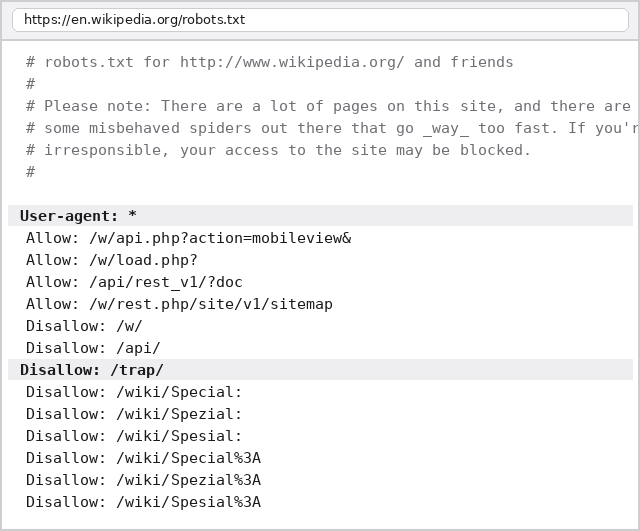
\includegraphics[width=\textwidth]{img/robots_txt_browser.png}
        \end{column}
    \end{columns}
    \bottomcite{Textbook Ch.~2, ``Comparing \texttt{robots.txt} Across Platforms.''}
\end{frame}

\begin{frame}{Activity: survey a sector}
    \begin{columns}[T]
        \begin{column}{0.6\textwidth}
            Three sites tell you little. A \textbf{sector} tells you about a business model. Take one row, fetch every \texttt{robots.txt} in it, and compare:
            \begin{itemize}\small
                \item \textbf{Search} --- \texttt{google.com}, \texttt{bing.com}, \texttt{duckduckgo.com}
                \item \textbf{Social} --- \texttt{facebook.com}, \texttt{instagram.com}, \texttt{linkedin.com}, \texttt{x.com}, \texttt{reddit.com}
                \item \textbf{Commerce} --- \texttt{amazon.com}, \texttt{ebay.com}, \texttt{ticketmaster.com}
                \item \textbf{Streaming} --- \texttt{netflix.com}, \texttt{hulu.com}, \texttt{spotify.com}
                \item \textbf{News} --- \texttt{nytimes.com}, \texttt{washingtonpost.com}, \texttt{wsj.com}, \texttt{theguardian.com}
                \item \textbf{Public} --- \texttt{leg.colorado.gov}, \texttt{census.gov}, \texttt{sec.gov}
            \end{itemize}
        \end{column}
        \begin{column}{0.35\textwidth}
            \begin{block}{Report back}
                \footnotesize
                \begin{itemize}\footnotesize
                    \item Most and least restrictive in your row?
                    \item What does the pattern say about \textbf{how each makes money}?
                    \item Does the \textbf{public} row look different --- and should it?
                \end{itemize}
            \end{block}
        \end{column}
    \end{columns}
    \bottomcite{Sector list adapted from the prior offering of this course. Count \texttt{Disallow} vs \texttt{Allow} lines with the loop from the last slide.}
\end{frame}

\begin{frame}{Which AI crawlers does this site block?}
    \begin{columns}[T]
        \begin{column}{0.6\textwidth}
            Since 2023, \texttt{robots.txt} has grown a second job: naming \textbf{AI training crawlers}. Search each file you fetched for:

            \smallskip
            {\footnotesize \texttt{GPTBot} (OpenAI) \textbar{} \texttt{ClaudeBot} (Anthropic) \textbar{} \texttt{CCBot} (Common Crawl) \textbar{} \texttt{Google-Extended} \textbar{} \texttt{Applebot-Extended} \textbar{} \texttt{Meta-ExternalAgent} \textbar{} \texttt{PerplexityBot}}

            \medskip

            Then look for the failure \textcite{koebler_wrong_2024} found: a site blocking a \textbf{retired} crawler name while the operator's \textbf{active} one walks straight through. Copy-pasted blocklists rot.

            \medskip

            \textbf{The deeper limit:} \texttt{robots.txt} has no enforcement mechanism. It is a sign on a door, not a lock --- \textcite{mehrotra_perplexity_2024} documents a company reaching blocked pages from an unpublicized IP address.
        \end{column}
        \begin{column}{0.35\textwidth}
            \begin{alertblock}{So why respect it?}
                \footnotesize Because you are not trying to get away with something --- you are trying to do defensible research.

                \smallskip

                The norm is weak against bad actors and completely effective against your reputation.
            \end{alertblock}
        \end{column}
    \end{columns}
    \bottomcite{Crawler-name rot: \textcite{koebler_wrong_2024}. Ignoring the protocol outright: \textcite{mehrotra_perplexity_2024}.}
\end{frame}

\begin{frame}[fragile]{Identify yourself, then slow down}
    Two habits make you a good citizen of the web --- a truthful \texttt{User-Agent} and rate limiting:
\begin{lstlisting}
import time, requests

headers = {
    "User-Agent": "WebDataScience/1.0 (INFO 4617; brian.keegan@colorado.edu)"
}

for url in urls:
    response = requests.get(url, headers=headers)
    # ... process the response ...
    time.sleep(1)          # a good default: about one request per second
\end{lstlisting}
    \begin{columns}[T]
        \begin{column}{0.6\textwidth}
            \footnotesize The default \texttt{requests} User-Agent marks you as an anonymous bot. A good one \textbf{identifies you and gives contact info}, so operators can reach you instead of simply blocking you --- and some APIs \textit{require} it. Hundreds of requests per second is an accidental \textbf{denial-of-service}: respect any \texttt{Crawl-delay} and stay well inside documented API limits.
        \end{column}
        \begin{column}{0.35\textwidth}
            \centering
            
\includegraphics[width=\textwidth]{img/user_agent_devtools.png}\\
            {\scriptsize Your header is visible to every server you touch.}
        \end{column}
    \end{columns}
    \bottomcite{Textbook Ch.~2, ``Responsible Request Headers'' \& ``Rate Limiting.'' HTTP mechanics: \textit{Missing Manual} Ch.~24.}
\end{frame}

\begin{frame}[fragile]{\texttt{responsible\_get()}: build it once}
    Custom User-Agent, rate limiting, and error handling appear in \textit{every} scraping project. Wrap them into one reusable function instead of re-implementing them ad hoc:
\begin{lstlisting}
import requests, time

def responsible_get(url, headers=None, delay=1.0):
    """GET with responsible defaults: identify, rate-limit, fail loudly."""
    default_headers = {
        "User-Agent": "WebDataScience/1.0 (INFO 4617; you@colorado.edu)"}
    if headers:
        default_headers.update(headers)
    try:
        response = requests.get(url, headers=default_headers, timeout=30)
        response.raise_for_status()      # treat 4xx/5xx as failures, not data
        time.sleep(delay)                # rate-limit by default
        return response
    except requests.exceptions.RequestException as e:
        print(f"Request failed ({type(e).__name__}): {url}")
        return None
\end{lstlisting}
    \bottomcite{Textbook Ch.~2, ``Building a Responsible Scraper Function.''}
\end{frame}

\begin{frame}{Why it's built that way --- and reused everywhere}
    \begin{columns}[T]
        \begin{column}{0.6\textwidth}
            \begin{block}{Every default encodes a principle}
                \begin{itemize}\small
                    \item \textbf{Custom User-Agent} --- identify \& give contact
                    \item \textbf{\texttt{delay} defaults ON} --- aggressive scraping must be a \textit{conscious} override, not an oversight
                    \item \texttt{raise\_for\_status()} --- a 403/404 fails loudly instead of feeding your parser garbage
                    \item broad \texttt{except} --- \texttt{ConnectionError}, \texttt{Timeout}, \texttt{SSLError} log rather than crash the run
                    \item \texttt{timeout=30} --- never hang forever on a dead server
                    \item pass a site's \texttt{Crawl-delay} as \texttt{delay} to honor its stated preference
                \end{itemize}
            \end{block}
        \end{column}
        \begin{column}{0.35\textwidth}
            \begin{alertblock}{You'll import this again}
                \footnotesize \texttt{responsible\_get()} returns in \textbf{Ch.~6} (scraping HTML tables), \textbf{Ch.~7} (Wayback snapshots), and throughout the \textbf{API chapters}.

                \medskip

                Building responsible defaults into your \textit{tools} is more reliable than remembering to add them each time.
            \end{alertblock}
        \end{column}
    \end{columns}
    \bottomcite{Textbook Ch.~2. Reused in later chapters on static pages, archives, and APIs.}
\end{frame}

\begin{frame}{Lab: work these, then show-and-tell}
    \begin{columns}[T]
        \begin{column}{0.6\textwidth}
            Work through the notebook exercises in pairs:
            \begin{enumerate}\small
                \item Compare \texttt{robots.txt} for five sites in one category --- what patterns emerge?
                \item ToS audit --- find three clauses restricting automated collection; do research exceptions apply?
                \item Run the five-question framework on a scenario: scraping a dating app's profiles to study self-presentation
                \item Rate-limit experiment --- time five requests with \texttt{time.time()} at 1s then 2s; does timing match intent?
                \item Audit a site you use daily: reconcile \texttt{robots.txt}, ToS, and the framework in 300 words --- where do they conflict?
                \item[6.] \textbf{5617}: read \textcite{fiesler2020no} + EFF's CFAA explainer + \textit{Van Buren}; write a two-page platform-collection memo
            \end{enumerate}
        \end{column}
        \begin{column}{0.35\textwidth}
            \begin{block}{Show-and-Tell}
                \footnotesize Come ready to share:
                \begin{itemize}\footnotesize
                    \item a challenging bug
                    \item interesting data you pulled
                    \item a provocation for a research design
                \end{itemize}
            \end{block}
        \end{column}
    \end{columns}
\end{frame}

\begin{frame}[standout]
    ``Can I scrape this?'' is the wrong question.\\[0.4em]
    Ask instead: \textit{should} I --- and if so, how do I do it responsibly?\\[1em]
    {\large Legality · Consent · Proportionality · Privacy · Server impact.}
\end{frame}

% =========================================================================
\section{Friday · Textbook Revisions}
% =========================================================================

\begin{frame}{Friday: your first contribution}
    \begin{columns}[T]
        \begin{column}{0.6\textwidth}
            Week 1 was a single short session and we ran out of room before anyone filed anything. So today we do it properly, and slowly.

            \medskip

            \textbf{By the end of class you will have:}
            \begin{enumerate}\small
                \item a working GitHub setup, verified with me in the room
                \item \textbf{one real issue filed} against Chapter~2
            \end{enumerate}

            \medskip

            Pull requests start \textbf{next week}. Today is the cheaper, faster half of contributing --- and it is the half that finds the problems.
        \end{column}
        \begin{column}{0.35\textwidth}
            \begin{tabular}{@{}ll@{}}
                \textbf{00:00 -- 00:06} & The four objects \\[0.2em]
                \textbf{00:06 -- 00:18} & Setup, together \\[0.2em]
                \textbf{00:18 -- 00:26} & What to look for \\[0.2em]
                \textbf{00:26 -- 00:32} & Anatomy of an issue \\[0.2em]
                \textbf{00:32 -- 00:47} & File it \\[0.2em]
                \textbf{00:47 -- 00:50} & Next week \\
            \end{tabular}
        \end{column}
    \end{columns}
    \bottomcite{Contributions \& reviews count toward the Textbook Revisions grade (15\%).}
\end{frame}

\begin{frame}{Four objects you'll use all semester}
    \begin{columns}[T]
        \begin{column}{0.6\textwidth}
            \begin{itemize}
                \item \textbf{Repository} --- the project: every file and its full history.
                \smallskip
                \item \textbf{Issue} --- a written report: ``here is a problem.'' Costs nothing but a browser.
                \smallskip
                \item \textbf{Pull request} --- a proposed change: ``here is the fix, side by side with the original.''
                \smallskip
                \item \textbf{Review} --- a response to a PR: comment line-by-line, then approve or request changes.
            \end{itemize}
        \end{column}
        \begin{column}{0.35\textwidth}
            \begin{block}{Issue vs.\ pull request}
                \footnotesize An \textbf{issue} says \textit{something is wrong}. A \textbf{pull request} says \textit{here is the correction} --- and shows the exact diff.
                \smallskip

                Issues are cheap and fast; PRs are the real contribution. \textbf{Today: an issue.} From next week on: pull requests.
            \end{block}
        \end{column}
    \end{columns}
    \bottomcite{This is how essentially all open-source software gets built --- including every library in this course.}
\end{frame}

\begin{frame}{Setup, together: two paths}
    \begin{columns}[T]
        \begin{column}{0.6\textwidth}
            \textbf{Filing an issue needs nothing but a browser} --- that is today, and it will work for everyone.

            \medskip

            But we are also getting your \textbf{tooling} working while I am standing here, so next week's pull-request day does not collapse. Pick one:

            \smallskip

            \textbf{GitHub Desktop} --- download, sign in, \textbf{Clone} the textbook repo. Everything after that is a button: branch, commit, push, Create Pull Request.

            \smallskip

            \textbf{The \texttt{gh} CLI} --- install, then \texttt{gh auth login}, then:
            {\footnotesize
            \begin{itemize}\footnotesize
                \item \texttt{gh repo clone cuinfoscience/Web-Data-Science-Book}
                \item \texttt{gh issue create} \quad(yes, you can file today's issue this way)
            \end{itemize}}
        \end{column}
        \begin{column}{0.35\textwidth}
            \begin{alertblock}{Checkpoint --- raise a hand}
                \footnotesize You are done when you can \textbf{see the textbook repo locally} in Desktop, or \texttt{gh repo clone} finishes without an error.

                \smallskip

                Do not silently fall behind here. This is the one class period where fixing it is free.
            \end{alertblock}
        \end{column}
    \end{columns}
    \bottomcite{Full instructions, both paths: \texttt{handouts/week-01/setup.md}. No raw \texttt{git} commands required in this course.}
\end{frame}

\begin{frame}{A revision menu for Chapter 2 --- pre-checked, ready to file}
    High-value targets --- pick one and scope it to a single PR:
    \begin{itemize}
        \item \textbf{A confirmed gap.} Wikipedia's live \texttt{robots.txt} now has a \texttt{Disallow: /trap/} rule the chapter doesn't mention --- a honeypot for bad bots. Explain what it's for and add it to the comparison.
        \item \textbf{Close a gap in ``Common Issues to Debug.''} Not covered yet: a blocked page can return \textbf{HTTP 200 with a Cloudflare challenge page}, not a 403 --- \texttt{raise\_for\_status()} won't catch it. Add this as a worked case.
        \item \textbf{Add a figure --- there are currently zero in this chapter.} A clean five-question framework diagram, an annotated \texttt{robots.txt} anatomy, or a CFAA case timeline.
        \item \textbf{Add a missing citation.} The Meta v.\ Bright Data (2024) and X Corp.\ rulings are described in prose with no source link --- find and add one.
        \item \textbf{Strengthen an exercise.} Add a rubric or expected output to the framework exercise (\#3), or a starter cell so it self-checks.
    \end{itemize}
    \bottomcite{Targets confirmed against the live chapter and current \texttt{robots.txt} --- not hypothetical.}
\end{frame}

\begin{frame}[fragile]{Anatomy of a good issue}
    \begin{columns}[T]
        \begin{column}{0.6\textwidth}
            Every issue you file this semester uses one skeleton:
\begin{lstlisting}[language=,basicstyle=\ttfamily\scriptsize]
Title:    <type>: <specific thing> in Ch. 2
Location: Section, and the file
          (ch-02-ethics.qmd)
Problem:  What you did, expected, got.
          Paste the code and output.
Why:      Who this affects. One sentence.
Proposal: The concrete change you'd make.
\end{lstlisting}

            \smallskip

            If you cannot fill in \textbf{Location} and \textbf{Problem} with specifics, you do not have an issue yet --- you have a hunch. Go back and reproduce it.
        \end{column}
        \begin{column}{0.35\textwidth}
            \begin{block}{Scored out of 10}
                \footnotesize
                \begin{itemize}\footnotesize
                    \item \textbf{Located} (2) --- section and file named
                    \item \textbf{Evidenced} (3) --- I can hit the same wall
                    \item \textbf{Actionable} (3) --- one concrete change
                    \item \textbf{Reviews} (2) --- from next week on
                \end{itemize}
            \end{block}
            \begin{alertblock}{Merged is not the bar}
                \footnotesize A well-evidenced issue I decline still earns full credit. A one-character typo fix does not.
            \end{alertblock}
        \end{column}
    \end{columns}
    \bottomcite{Full rubric and worked examples: \texttt{handouts/common/revision-framework.md}}
\end{frame}

\begin{frame}{File it: your first issue}
    \begin{columns}[T]
        \begin{column}{0.6\textwidth}
            \textbf{Fifteen minutes. Everyone files one.}

            \medskip

            \begin{enumerate}
                \item Open \texttt{ch-02-ethics.qmd} in the textbook repo --- or the rendered chapter, whichever you prefer to read.
                \item Find one thing from the revision menu, or anything else that genuinely tripped you.
                \item Reproduce it. Copy the exact passage, command, or output.
                \item \textbf{Issues} tab $\rightarrow$ \textbf{New issue} $\rightarrow$ fill in the skeleton $\rightarrow$ \textbf{Submit}.
                \item Paste your issue URL into the Canvas assignment.
            \end{enumerate}

            \medskip

            Check open issues first --- if someone already filed yours, \textbf{say so in a comment} and add what they missed. That counts.
        \end{column}
        \begin{column}{0.35\textwidth}
            \centering
            
\includegraphics[width=\textwidth]{img/github_issue.png}\\
            {\scriptsize One browser tab. No install required.}
        \end{column}
    \end{columns}
    \bottomcite{Due tonight at midnight if you do not finish in class --- but the point is that you finish in class.}
\end{frame}

\begin{frame}{Next week: from issues to pull requests}
    \begin{columns}[T]
        \begin{column}{0.6\textwidth}
            An issue says \textit{something is wrong}. Starting next week you say \textit{here is the fix} --- and back it with a diff.

            \medskip

            \begin{block}{A strong PR}
                \begin{itemize}\small
                    \item One focused change, clearly titled
                    \item Explains the problem it fixes
                    \item Builds (\texttt{quarto render}) without errors
                    \item Matches the book's voice and notation
                    \item Discloses any AI assistance
                \end{itemize}
            \end{block}
        \end{column}
        \begin{column}{0.35\textwidth}
            \begin{block}{A strong review}
                \begin{itemize}\small
                    \item Runs / reads the change, not just skims
                    \item Names specifics (line, claim, code)
                    \item Separates ``must fix'' from ``nice to have''
                    \item Is generous --- assume good faith
                    \item Ends with a clear verdict
                \end{itemize}
            \end{block}
        \end{column}
    \end{columns}
    \medskip
    \centering\small Next week: \textbf{The Post-API Age} --- why the open web is closing, and how researchers adapt.
\end{frame}

% =========================================================================
\begin{frame}{Key takeaways}
    \begin{enumerate}
        \item \textbf{``Can I?'' is not ``should I?''} --- the real question is how to collect data \textit{responsibly}.
        \item The law is unsettled: the CFAA targets \textbf{bypassing gates} (Van Buren), but \textbf{contracts and ToS} still bite (hiQ); state privacy laws and GDPR reach personal data.
        \item \texttt{robots.txt} is a \textbf{norm, not a law} --- read it, respect \texttt{Disallow} and \texttt{Crawl-delay}; a 404 means no rules, not open season.
        \item \textbf{Identify yourself} (custom \texttt{User-Agent}) and \textbf{rate-limit} (\texttt{time.sleep}) --- then wrap both into \texttt{responsible\_get()} and reuse it.
        \item Run the \textbf{five-question framework} before every project; when in doubt, use an API, collect less, and err toward caution.
    \end{enumerate}
    \bigskip
    \bottomcite{Reading: Textbook Ch.~2. Related: \textcite{fiesler2020no}; \textcite{freelon2018computational}.}
\end{frame}

\end{document}
